\def\year{2016}\relax
\documentclass[letterpaper]{article}
\usepackage{aaai16}
\usepackage{times}
\usepackage{helvet}
\usepackage{courier}
\frenchspacing
\setlength{\pdfpagewidth}{8.5in}
\setlength{\pdfpageheight}{11in}
\usepackage{url}
\usepackage[round]{natbib}
\usepackage{amsmath,amsfonts,amssymb,bm,graphicx,amsthm}
\usepackage{subfig}
\usepackage{wrapfig}
\usepackage{dblfloatfix}
\renewcommand\textfraction{.1}
\setlength{\abovecaptionskip}{2pt}
\setlength{\belowcaptionskip}{2pt}
\setlength{\floatsep}{2pt}
\setlength{\textfloatsep}{2pt}
\usepackage{t1enc} % as usual
\usepackage[utf8]{inputenc} % as usual
\usepackage[french]{babel}
\usepackage{makeidx}
\usepackage[titletoc]{appendix}
\usepackage[shortlabels]{enumitem} 
\usepackage{listingsutf8}
\usepackage{csquotes}
\usepackage[table]{xcolor}
\usepackage{xspace}
\usepackage{multirow}
\usepackage{siunitx}
\usepackage{hyperref}
\usepackage{xparse}
\usepackage{mathtools, stmaryrd}
\usepackage[T1]{fontenc}

\usepackage[colorinlistoftodos,prependcaption,textsize=tiny]{todonotes}

\hypersetup{
    colorlinks  = true,
    linkcolor   = black,
    citecolor   = blue,
    urlcolor    = blue,
    linktocpage = false
}

\nocopyright

\pdfinfo{
/Title (Cooperative Pathfinding)
/Author (Angelo Ortiz)
}
\setcounter{secnumdepth}{0}

\graphicspath{ {../img/} }
\begin{document}


\title{Cooperative Pathfinding}

\author{Angelo Ortiz \\
Sorbonne Universit\'e}

\hyphenation{Zaxxon Double}

\maketitle

\section{Introduction}
De nos jours, c'est un fait que les robots se sont r\'epandus dans les industries et ils ont ainsi remplac\'e, parfois compl\`etement, l'humain dans certaines t\^aches. 
Par exemple, ils sont de plus en plus utilis\'es dans les actes chirurgicaux, comme la laparoscopie, du fait de leur pr\'ecision.
Pour d'autres t\^aches, comme le d\'eplacement de marchandises ou des objets lourds dans les usines, il est aussi plus int\'eressant de les affecter aux robots.

Mettons-nous dans cette derni\`ere situation.
Nous avons une entreprise qui compte plusieurs robots charg\'es de d\'eplacer des marchandises \`a l'int\'erieur d'une usine. 
Il est \'evident que l'objectif est d'effectuer des d\'eplacements de mani\`ere efficiente, i.e.\ des trajets plus courts. 
Supposons de plus que les objets \`a ramasser soient r\'epartis entre l'ensemble de robots de sorte qu'il n'y ait qu'un seul robot ciblant un objet.

La premi\`ere r\'eponse na\"ive au probl\`eme des d\'eplacements est de calculer, pour chaque entit\'e, le plus court chemin \`a son but compte tenu des obstacles et de les faire emprunter ces chemins.
En effet, plusieurs algorithmes de tr\`es bonne complexit\'e temporelle  sont connus \`a cet effet.
Cependant, nous nous apercevons que cette approche n'est pas efficace car elle n\'eglige les potentielles collisions qui peuvent survenir en cours de route.

Cela nous am\`ene \`a concevoir une autre strat\'egie tenant compte des possibles collisions pour r\'esoudre ce probl\`eme.
Il s'agit ainsi du probl\`eme de la recherche coop\'erative (en anglais \textit{Cooperative Pathfinding}).

Dans le cadre de l'UE 3I025 - Introduction \`a l'intelligence artificielle et la recherche op\'erationnelle, le sujet du premier mini-projet propos\'e prend la forme du probl\`eme du \textit{Cooperative Pathfinding} et il consiste \`a r\'esoudre ce probl\`eme au travers des diff\'erentes strat\'egies appel\'ees \textit{opportuniste}, \textit{coop\'erative de base} et \textit{coop\'erative avanc\'ee}.

Dans la suite de ce document, je vais expliquer en d\'etail les sp\'ecifications du sujet, mes choix d'impl\'ementation et commenter mes r\'esultats obtenus.

\section{Pr\'esentation}
Dans le cadre de ce projet, le probl\`eme du \textit{Cooperative Pathfinding} prend la forme d'une grille rectangulaire \`a deux dimensions.
Elle comporte trois types d'objets : les joueurs, les fioles et les murs.
Un joueur peut se d\'eplacer sur la carte, prendre une fiole s'il y en a une sur sa case, mais ne peut pas traverser les murs ni les autres joueurs, ce que l'on appelera une \textit{collision}.

Trois types de collisions ont \'et\'e d\'efinis :
\begin{enumerate}[(I)]
 \item la \textit{concurrence}, o\`u deux agents veulent tous les deux se diriger vers la m\^eme position \`a l'instant suivant ;
 \item le \textit{croisement}, o\`u deux agents se traversent l'un l'autre en un instant de temps ;
 \item la \textit{poursuite}, o\`u un agent se dirige vers un emplacement d\'ej\`a occup\'e par un autre agent qui avance dans son chemin en ne traversant le premier agent. 
\end{enumerate}
Les deux premi\`eres collisions sont dites \textit{frontales}, puisqu'elles n'arrivent que lorsque les deux agents se trouvent face \`a face.

Par ailleurs, le probl\`eme a \'et\'e consid\'er\'e comme \'etant \`a information compl\`ete. 
Autrement dit, les agents connaissent l'int\'egralit\'e de la carte, ce qui correspond \`a l'emplacement des obstacles, et la position de leurs pairs et leurs tr\'esors associ\'es.
Nonobstant, un joueur ne peut r\'ecup\'erer que la fiole qui lui a \'et\'e associ\'e au d\'epart.

Le but est alors de trouver les plus courts chemins des agents \`a leur fiole respective tout en \'evitant les collisions entre les agents.
\`A cet effet, trois strat\'egies ont \'et\'e propos\'ees : la strat\'egie opportuniste, la coop\'eration de base et la coop\'eration avanc\'ee.

Il est important de remarquer que l'ordre de passage des agents est d\'efini et fix\'e lors de l'instanciation du probl\`eme : il correspond \`a l'ordre de cr\'eation des agents.

\section{Strat\'egies}
La base de toutes mes strat\'egies de r\'esolution du probl\`eme du \textit{Cooperative Pathfinding} est la recherche du plus court chemin dans une carte avec obstacles. 
Pour ce faire, j'ai utilis\'e l'algorithme A*.
Puis, j'ai impl\'ement\'e trois fa\c{c}ons de g\'erer les potentielles collisions sur la carte : elles correspondent aux strat\'egies d\'etaill\'ees dans les sections qui suivent.

Pour la premi\`ere et la troisi\`eme approche, les agents g\`erent uniquement les collisions frontales pour faciliter le recalcul de chemin. 
Quant \`a la deuxi\`eme, les trois types de collisions ont \'et\'e consid\'er\'es du fait de sa conception stricte.

Une caract\'eristique importante des impl\'ementations que j'ai r\'ealis\'ees est qu'elles supportent la recherche successive de fioles pour les agents.
Il s'agit en fait du but cherch\'e tout au long du mini-projet.

Pour la premi\`ere et la troisi\`eme strat\'egie, j'ai m\^eme rajout\'e la fonctionnalit\'e d'accepter une liste de fioles \`a traiter.
Deux strat\'egies ont \'et\'e d\'evelopp\'ees pour g\'erer ce cas de figure : la premi\`ere est na\"ive et consid\`ere les fioles dans leur ordre dans la liste ; la deuxi\`eme, en revanche, correspond \`a un comportement \textit{de proche en proche}.
Dans le cadre du projet, seulement la premi\`ere d'entre elles \`a \'et\'e utilis\'ee.

\subsection{Opportunisme}
La premi\`ere strat\'egie, dite \textit{opportuniste}, consiste \`a d\'emarrer le chemin de tous les agents en m\^eme temps et de g\'erer les collisions lorsqu'elles sont imminentes.
Pour ce faire, j'ai utilis\'e la m\'ethode connue comme \textit{path splicing}.

Lorsqu'un agent d\'etecte que la suite de son chemin l'am\`ene vers une collision \`a l'instant suivant, il d\'ecide de recalculer une partie de son chemin.
Pour ce faire, il utilise de nouveau l'algorithme A* jusqu'au bout de la portion de chemin \`a remplacer en tenant compte des positions bloqu\'ees par la collision.
Puis, il joint les deux morceaux de chemin et suit le chemin cr\'e\'e.
Ce comportement implique que la gestion des collisions est laiss\'ee \`a la charge du premier agent (dans l'ordre de passage) concern\'e.

J'ai trouv\'e deux points importants \`a remarquer dans cette m\'ethode.
D'une part, la longueur de la portion de chemin \`a recalculer joue un r\^ole crucial.
En effet, si l'agent est amen\'e \`a calculer des longs morceaux de chemin et que les collisions sont fr\'equentes, il passera la majorit\'e de son temps \`a faire des calculs inutiles, puisqu'il ne suivra qu'une infime partie des chemins calcul\'es.
C'est pourquoi, tout au long de mes tests, j'ai fix\'e la \textit{longueur de coupure} \`a 5.

D'autre part, il se peut que le chemin restant pour atteindre la fiole respective ne soit pas plus long que la longueur de coupure fix\'ee.
Dans ce cas, l'agent supprime son chemin restant et fait un pas al\'eatoire valide dans l'une des positions adjacentes, y compris sa position courante.
Il s'av\`ere que cette \textit{randomisation} all\`ege le temps de calcul et simplifie la conduite par la suite, \'etant donn\'e qu'elle repousse la recherche du chemin restant \`a l'instant suivant o\`u les agents concern\'es se trouvent dans d'autres positions.
De plus, le pas al\'eatoire est tr\`es utile lorsque la position de collision se trouve dans une zone concentr\'ee d'agents, et surtout lorsqu'il est nul, i.e.\ l'agent reste immobile, dans quel cas le co\^ut associ\'e est 0.

\subsection{Coop\'eration na\"ive}
La deuxi\`eme m\'ethode, dite de \textit{planification}, correspond \`a la strat\'egie qui lance en parall\`ele les agents dont les chemins ne partagent aucune case. 

J'ai d\'efini une entit\'e appel\'e \textit{planifieur}, qui commande et fixe l'ordre de passage des agents.
Tout d'abord, tout agent calcule son chemin optimal comme s'il \'etait le seul agent sur la carte.
Puis, le planifieur d\'etermine les groupes d'agents dont les chemins ne se croisent pas. De cette mani\`ere, tous les membres d'un groupe peuvent d\'emarrer leur chemins sans crainte de collision.

Il est important de noter que s'il y a un agent qui se trouve sur le chemin optimal d'un autre agent et que c'est ce dernier qui passe en premier, alors le deuxi\`eme agent entrera en collision avec le premier.
Pour \'eviter ce cas de figure, les agents d\'eterminent leurs chemins optimaux en consid\'erant les positions initiales de leurs pairs comme des obstacles.

Le m\^eme probl\`eme arrive avec les positions finales des agents qui ont d\'ej\`a r\'eussi \`a r\'ecup\'erer leur fiole : le reste n'avait pas pr\'evu le nouveau emplacement du premier groupe et il y a ainsi un risque de collision.
J'ai remarqu\'e que rajouter la position finale des agents dans la recherche initiale du chemin optimal complique la situation, notamment lorsque la fiole d'un agent se trouve sur une case \'etant la seule \textit{porte} pour une zone de cases contenant la fiole d'un autre agent.
J'ai donc d\'ecid\'e de faire un compromis entre l'efficacit\'e et le temps d'ex\'ecution : une fois le premier groupe pass\'e, les agents restants recalculent leurs chemins avec les positions courantes de leurs pairs, et les groupes peuvent donc varier.

Par ailleurs, je n'ai pas encore pr\'ecis\'e le crit\`ere pour l'ordre de passage des groupes. \`A cet effet, deux strat\'egies ont \'et\'e impl\'ement\'ees : les groupes les plus rapides d'abord, et les groupes les plus nombreux d'abord.

\begin{figure}[!h]
  \centering
  \captionsetup{justification=centering}
  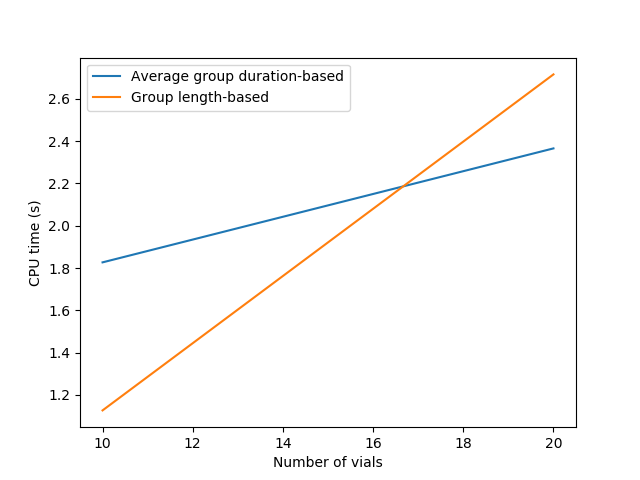
\includegraphics[width=0.5\textwidth]{planner_cpu_time}
  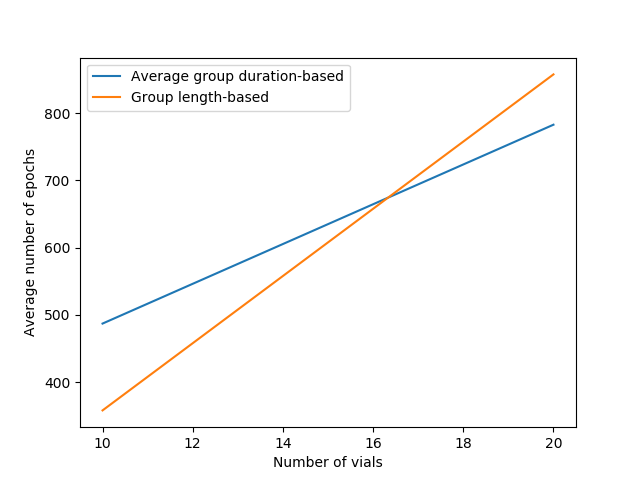
\includegraphics[width=0.5\textwidth]{planner_epoch}
  \caption{Comparaison des deux strat\'egies d'ordonnancement des groupes pour la m\'ethode de \textit{planification}}
  \label{fig:1j}
\end{figure}

Comme vous pourrez appr\'ecier dans la figure \ref{fig:1j}, lorsque le nombre de fioles \`a ramasser devient plus important, il est pr\'ef\'erable de faire passer en premier les groupes dont le nombre de pas moyens est plus petit.

Finalement, la derni\`ere sp\'ecificit\'e de cette impl\'ementation est que pour r\'eduire la possibilit\'e de famine, les agents du dernier groupe commencent leur recherche d'un nouveau groupe \`a partir de la fin de la s\'equence d\'efinie pour les autres.

\subsection{Coop\'eration avanc\'ee}
Finalement, la troisi\`eme approche, dite \textit{avanc\'ee}, est une impl\'ementation de l'algorithme \textit{Windowed Hierarchical Cooperative A*} propos\'e par David Silver. %\citet{}

Dans cette approche, la carte des joueurs devient un espace tridimensionnel o\`u le temps a \'et\'e rajout\'e.
De plus, l'heuristique de la distance de Manhattan est remplac\'ee par la distance r\'eelle entre toute position et l'objectif.
Pour ce faire, j'ai utilis\'e une version modifi\'ee de l'algorithme A* spatial o\`u la position initiale est celle de la fiole cherch\'ee et dont l'objectif peut \^etre modifi\'e en cours d'ex\'ecution.
Ceci a r\'eduit le temps mis par les it\'erations de A* tridimensionnel car il stocke en m\'emoire la recherche de A* spatial et n'a donc besoin de le relancer que lorsqu'un n\oe ud pas encore visit\'e est atteint.

En ce qui concerne la gestion des collisions, une table de r\'eservation des positions  dans le temps est mise en place.
Lorsqu'un joueur lance sa recherche de A* spatio-temporel, il consid\`ere les positions r\'eserv\'ees par ses pairs dans la table et r\'eserve lui-m\^eme les cases correspondant \`a son chemin optimal.
Au contraire de la strat\'egie opportuniste, un agent n'encourt aucun co\^ut s'il reste immobile et il a d\'ej\`a atteint son but.

Comme la recherche de A* invers\'e est stock\'ee en m\'emoire, il est raisonnable de l'effectuer par morceaux.
De plus, tous les agents anticipent les collisions, et donc certaines mesures lointaines peuvent ne pas \^etre n\'ecessaires lorsque arriv\'es \`a ce point, ce qui les rend inutiles.
De ces faits, la recherche d'un agent est effectu\'ee par \textit{fen\^etre fixe} : elle n'est pas ex\'ecut\'ee jusqu'\`a l'atteignement du but, mais pour un nombre de pas fix\'es appel\'e \textit{fen\^etre}, et ce, m\^eme si l'agent arrive \`a la position de sa fiole avec moins de pas.

Pour que ces recherches soient efficientes, mais que la pr\'esence de l'agent dans la table de r\'eservation reste consid\'erable, j'ai fix\'e la \textit{fr\'equence de recherche} \`a la moiti\'e de ladite fen\^etre.
Cependant, cette m\'ethode reste encore sous-optimale du fait que les derniers agents \`a passer ne disposent que d'un nombre limit\'e de choix lors de leurs recherches.
Pour y rem\'edier, les recherches sont intercal\'ees. 

Les agents sont class\'es dans divers groupes comportant \`a peu pr\`es le m\^eme nombre de joueurs de telle sorte qu'\`a chaque instant, un seul groupe fasse sa recherche. 
Cette m\'ethode circulaire r\'eduit le d\'esavantage d'un agent \`a son groupe, puisque cet ensemble sera \`a un moment le premier \`a r\'eserver des positions.
En outre, cette approche am\'eliore la coop\'eration des agents parce que l'agent qui a d\'ej\`a r\'eussi son but se verra oblig\'e de se d\'ecaler dans son avenir proche lorsque l'un des autres aura r\'eserv\'e au pr\'ealable la position sur laquelle il se trouve actuellement.

J'ai constat\'e que la valeur de la fr\'equence des recherches a un gros impact sur la performance de cette strat\'egie.
En effet, les agents \`a l'int\'erieur d'un groupe effectuent leurs recherches dans le m\^eme ordre, ce qui fait que lorsque les premiers ont d\'ej\`a r\'eussi leurs objectifs et bloquent la route optimale des derniers, ceux-ci peinent \`a trouver la bonne voie. Leur comportement se r\'eduit alors \`a avancer et reculer d'un pas de mani\`ere altern\'ee, et ils n'arrivent donc pas \`a franchir cette barri\`ere.

J'ai trouv\'e que pour des valeurs de fr\'equences inf\'erieures au nombre d'agents, il y a un risque consid\'erable de non terminaison pour les derniers agents appartenant \`a un groupe nombreux. Au contraire, pour des valeurs beaucoup plus grandes que le nombre de joueurs, les agents effectuent des longues recherches, et le temps CPU et le nombre de pas n\'ecessaires, tous les agents confondus, deviennent importants.

\section{Exp\'erimentation}
Je m'attendais \`a que la m\'ethode la plus performante en nombre moyen de fioles ramass\'ees soit la troisi\`eme, suivie de la premi\`ere et, enfin, la deuxi\`eme.
En effet, la table de r\'eservation est assez costaude et permettrait de surclasser le \textit{path splicing}.
De plus, il est \'evident que la deuxi\`eme, de par le lancement en differ\'e, est la moins performante.

Cependant, dans la table \ref{tab:stats}, vous pouvez remarquer que la m\'ethode optimale est la premi\`ere.
Ceci peut \^etre expliqu\'e par le fait que les cartes utilis\'ees sont encore de taille raisonnable pour l'utilisation du \textit{path splicing}.
Les effets de la m\'ethode avanc\'ee, qui a \'et\'e con\c{c}ue pour des probl\`emes plus complexes, notamment lorsque le nombre de joueurs est consid\'erable, restent ainsi mod\'er\'es.

\begin{table}
    \centering
    \begin{tabular}{|c|c|c|}
	\hline Strat\'egie & Temps CPU (en \si{s}) & Nombre de fioles \\ 
    \hline Opportuniste & 0.425 & 29.3 \\ 
	\hline Planification & 0.595 & 3.33 \\ 
	\hline Avanc\'ee & 4.29 & 21.3 \\ 
	\hline
	\end{tabular}
	\caption{Statistiques sur les performances des trois strat\'egies pour un nombre de pas fix\'e \`a 200 et la carte \`a 6 joueurs}
  \label{tab:stats}
\end{table}

\section{Conclusion}
Dans le cadre de ce mini-projet, j'ai impl\'ement\'e un algorithme de recherche de chemin optimal dans un carte avec obstacles, et je l'ai utilis\'e pour r\'epondre au probl\`eme du \textit{Cooperative Pathfinding}.
Pour ce faire, je l'ai enrichi \`a travers diff\'erentes m\'ethodes.
Ces m\'ethodes avaient chacune leurs particularit\'es et m'ont donn\'e des r\'esultats assez vari\'es.

Ce mini-projet m'a aid\'e \`a renforcer mes connaissances en recherche de chemin optimaux et, surtout, m'a fait r\'ealiser que l'on rencontre toujours des situations sortent du cadre et qu'il faut \^etre pr\'epar\'es et capables de les traiter de mani\`ere flexible.

\end{document}



